\documentclass[conference]{IEEEtran}
\IEEEoverridecommandlockouts
% The preceding line is only needed to identify funding in the first footnote. If that is unneeded, please comment it out.
\usepackage{cite}
\usepackage{amsmath,amssymb,amsfonts}
\usepackage{algorithmic}
\usepackage{graphicx}
\graphicspath{{figures/}{./}}
\usepackage{textcomp}
\usepackage{xcolor}
\usepackage{booktabs}
\usepackage{url}
\usepackage{microtype}

\def\BibTeX{{\rm B\kern-.05em{\sc i\kern-.025em b}\kern-.08em
    T\kern-.1667em\lower.7ex\hbox{E}\kern-.125emX}}

\begin{document}

\title{Autonomous Multi-Agent Portfolio Management System (AD-COP): Decoupling Adversarial Qualitative LLM Debate from Convex Optimization with Layered Vector Memory and Decontaminated Contamination Shield}

\author{\IEEEauthorblockN{Vibhor Shukla}
\IEEEauthorblockA{\textit{Department of Computer Science and Engineering} \\
\textit{National Institute of Technology (NIT) Raipur}\\
Raipur, Chhattisgarh, India \\
Email: vshukla107.btech2023@cse.nitrr.ac.in}
}

\maketitle

\begin{abstract}
Direct capital allocation via generative Large Language Models (LLMs) suffers from three recurring failure modes: autoregressive weight hallucinations that violate simplex constraints, insensitivity to empirical cross-asset covariance matrices, and unmonitored look-ahead bias originating from pre-training memorization. In this study, we present the Adversarial Debate and Convex Optimization Portfolio (AD-COP) system, an algorithmic asset management architecture that strictly decouples qualitative linguistic reasoning from numerical convex portfolio optimization. Our framework organizes specialized agents into an adversarial Bull-Bear debate adjudicated by an impartial orchestrator, informed by a three-tier semantic vector memory with layer-specific exponential half-lives. Rather than predicting raw portfolio allocations, the qualitative agents produce bounded expected return vectors that feed into Bayesian Black-Litterman and Hierarchical Risk Parity solvers. To systematically investigate historical data contamination, we introduce the DECONTAM protocol, an entity and date anonymization harness that scrubs corporate and temporal identifiers during backtesting. Benchmarking across a six-month crisis horizon (November 2022 to May 2023 across five volatile equities) that contextualizes the asset universe of prior studies, our decontaminated pipeline achieves a discrete return of +24.45\% and an annualized Sharpe ratio of 0.77 (maximum drawdown of -17.11\%), outperforming the Equal-Weight benchmark (+3.28\%) and the S\&P 500 (+8.97\%) under strict blind conditions. A comparative ablation reveals a +16.29\% look-ahead premium when models operate on unmasked historical feeds, indicating that previously published single-model trading benchmarks substantially inflate alpha through memorized post-event trajectories.
\end{abstract}

\begin{IEEEkeywords}
Multi-Agent Systems, Convex Optimization, Black-Litterman Model, Large Language Models, Look-Ahead Bias, Algorithmic Trading, Hierarchical Risk Parity.
\end{IEEEkeywords}

\section{Introduction}

Algorithmic asset management operates at the intersection of two conflicting data modalities: unstructured qualitative narratives (corporate regulatory filings, earnings calls, news headlines) and structured quantitative series (historical price returns, covariance matrices, volatility surfaces). Classical quantitative finance models, such as Markowitz mean-variance optimization \cite{markowitz1952} and risk parity, excel at processing covariance structures but remain completely blind to corporate events, earnings revisions, and macroeconomic policy shifts.

Recent initiatives have applied Large Language Models (LLMs) directly to financial asset allocation \cite{wu2023bloomberg, yu2023finmem, xiao2024tradingagents}. However, treating portfolio construction as an autoregressive text generation problem introduces critical structural bugs:

\begin{enumerate}
    \item \textbf{Simplex Constraint Violations:} Autoregressive text generation cannot guarantee that output weight vectors satisfy the fundamental allocation constraint $\sum_{i=1}^N w_i = 1$ with $w_i \ge 0$ for long-only portfolios. In production runs, naive prompting frequently outputs negative weights, unallocated cash, or weights exceeding unity.
    \item \textbf{Covariance Blindness:} Natural language models evaluate assets in qualitative isolation. When prompted on multiple equities, they allocate heavily to whatever assets show strong narrative momentum, entirely ignoring empirical cross-asset covariance $\Sigma$. This causes dangerous overconcentration in correlated high-beta assets.
    \item \textbf{Narrative Sycophancy:} Unconstrained prompting exhibits strong confirmation bias when processing corporate public relations statements, uncritically accepting forward management guidance while discounting balance sheet leverage and credit strain.
    \item \textbf{Parametric Look-Ahead Memorization:} Most foundation models have pre-training data that overlaps with commonly backtested historical windows (e.g., 2022--2023). When given unmasked ticker symbols, models exploit memorized historical trajectories, creating an illusion of forecasting skill that deteriorates out of sample.
\end{enumerate}

To resolve these contradictions, we design the AD-COP framework based on a strict separation of concerns: \textit{agents handle qualitative argumentation, while numerical convex solvers handle portfolio weight optimization}. Qualitative consensus from an adversarial Bull-Bear debate is mapped onto bounded expected return vectors $Q$, which then serve as subjective views in a Bayesian Black-Litterman solver \cite{black1992} or fall back to Hierarchical Risk Parity \cite{prado2016} when covariance matrices approach singularity.

We also investigate the pervasive issue of look-ahead contamination in financial AI benchmarks. Using an entity and temporal anonymization protocol termed DECONTAM, we directly measure the return differential between unmasked backtests and genuine blind simulations. Our contributions are summarized as follows:

\begin{itemize}
    \item We formulate the AD-COP decoupled architecture where adversarial multi-agent debate produces structured Bayesian views rather than continuous portfolio weights, eliminating autoregressive allocation hallucinations.
    \item We construct a three-tier semantic vector memory engine that differentiates transient sentiment noise from multi-quarter macroeconomic regimes using calibrated exponential decay rates.
    \item We design the DECONTAM entity and date anonymization protocol that establishes a reproducible method for measuring parametric look-ahead contamination in LLM financial benchmarks.
    \item We empirically isolate a +16.29\% look-ahead bias premium on a standardized six-month test universe, demonstrating that our decontaminated pipeline maintains positive risk-adjusted alpha (+24.45\% return, Sharpe 0.77) under 100\% blind conditions.
\end{itemize}

\section{Theoretical Foundations and Related Work}

\subsection{Modern Portfolio Theory and Estimation Sensitivity}

Let a portfolio consist of $N$ risky assets with return vector $R = [R_1, \dots, R_N]^T \sim \mathcal{N}(\mu, \Sigma)$, where $\mu \in \mathbb{R}^N$ represents expected excess returns and $\Sigma \in \mathbb{R}^{N \times N}$ is the covariance matrix. The portfolio return is $R_p = w^T R$ with variance $\sigma_p^2 = w^T \Sigma w$, constrained to the simplex $\Delta^N = \{w \in \mathbb{R}^N : \sum_{i=1}^N w_i = 1, w_i \ge 0\}$.

The classic Markowitz formulation \cite{markowitz1952} maximizes risk-adjusted utility:
\begin{equation}
\max_{w \in \Delta^N} \left( w^T \mu - \frac{\lambda}{2} w^T \Sigma w \right)
\label{eq:markowitz}
\end{equation}
where $\lambda > 0$ is the risk-aversion parameter. The unconstrained analytical solution requires inverting the sample covariance matrix, $w^* = \frac{1}{\lambda} \hat{\Sigma}^{-1} \hat{\mu}$. As Michaud demonstrated \cite{michaud1989}, sample inversion acts as an estimation error amplifier: assets with artificially high sample means or understated variances receive extreme long positions, whereas modest estimation errors produce volatile out-of-sample performance that frequently lags equal-weighting \cite{demiguel2009}.

\subsection{The Black-Litterman Bayesian Updating Model}

The Black-Litterman model \cite{black1992, he1999} stabilizes the optimization problem by anchoring expectations to a Capital Asset Pricing Model (CAPM) equilibrium prior. By reverse-optimizing benchmark market capitalization weights $w_{\text{mkt}}$, the implied equilibrium return vector $\Pi$ is extracted:
\begin{equation}
\Pi = \lambda \Sigma w_{\text{mkt}}
\label{eq:bl_prior}
\end{equation}
where $\lambda$ represents market risk aversion. The prior distribution over mean returns is expressed as $\mu \sim \mathcal{N}(\Pi, \tau \Sigma)$, with scalar $\tau = 0.05$ denoting uncertainty in the prior.

Subjective qualitative analyst views are represented as $K$ linear equations:
\begin{equation}
P \mu = Q + \varepsilon, \quad \varepsilon \sim \mathcal{N}(0, \Omega)
\label{eq:bl_views}
\end{equation}
where $P \in \mathbb{R}^{K \times N}$ maps views to specific assets, $Q \in \mathbb{R}^K$ contains expected return values, and $\Omega \in \mathbb{R}^{K \times K}$ is a diagonal matrix of view uncertainties. Following He and Litterman \cite{he1999}, uncertainty scales with prior asset variance:
\begin{equation}
\Omega = \text{diag}\left(P (\tau \Sigma) P^T\right)
\label{eq:omega}
\end{equation}
Bayesian generalized least squares updating yields the conditional posterior distribution $\mu_{\text{BL}} \sim \mathcal{N}(E(R), M)$:
\begin{equation}
E(R) = \left[(\tau \Sigma)^{-1} + P^T \Omega^{-1} P\right]^{-1} \left[(\tau \Sigma)^{-1} \Pi + P^T \Omega^{-1} Q\right]
\label{eq:bl_posterior}
\end{equation}
\begin{equation}
M = \Sigma + \left[(\tau \Sigma)^{-1} + P^T \Omega^{-1} P\right]^{-1}
\label{eq:bl_cov}
\end{equation}
The resulting posterior expected returns $E(R)$ and covariance $M$ are passed to a convex quadratic solver to identify the maximum Sharpe ratio allocation.

\subsection{Hierarchical Risk Parity (HRP)}

When cross-asset correlations are high, the empirical covariance matrix $\Sigma$ exhibits ill-conditioning, with matrix condition numbers $\kappa(\Sigma) \gg 10^3$. Under these conditions, numerical matrix inversion introduces substantial rounding noise. Hierarchical Risk Parity \cite{prado2016} replaces matrix inversion with unsupervised graph partitioning across three phases:
\begin{enumerate}
    \item \textbf{Tree Clustering:} Pairwise correlation coefficients $\rho_{i,j}$ are converted into distance metrics $d_{i,j} = \sqrt{\frac{1}{2}(1 - \rho_{i,j})}$. A hierarchical cluster tree is formed via Ward's minimum-variance linkage.
    \item \textbf{Quasi-Diagonalization:} The covariance matrix rows and columns are sorted to place contiguous risk clusters adjacent along the diagonal.
    \item \textbf{Recursive Bisection:} Portfolio capital is allocated top-down by splitting clusters into sub-clusters $(C_1, C_2)$ using split variance ratios:
    \begin{equation}
    \alpha_1 = 1 - \frac{V_1}{V_1 + V_2}, \quad V_k = w_k^T \Sigma_k w_k
    \label{eq:hrp_bisection}
    \end{equation}
    where $w_k$ denotes inverse-variance cluster weights.
\end{enumerate}

\subsection{Related Work in Financial LLM Agents}

Recent investigations into financial LLMs have expanded rapidly. Yu et al. introduced \textit{FinMem} \cite{yu2023finmem}, applying layered cognitive memory and character personas to single-asset trading. While FinMem demonstrated that memory improves signal retention over reinforcement learning baselines, it trades assets in complete isolation, precluding portfolio-level covariance modeling. Xiao et al. proposed \textit{TradingAgents} \cite{xiao2024tradingagents}, introducing adversarial Bull-Bear debate to curb single-agent optimism, but relied on direct natural language output for final trade decisions without a numerical optimizer. Lee et al. \cite{lee2025llmbl} examined linking single LLMs to Black-Litterman models, but omitted adversarial debate and memory decay mechanisms. Guo et al. \cite{guo2024mass} explored population scaling across 512 heterogeneous simulation agents in their framework named MASS, but did not incorporate convex quadratic optimizers, adversarial debate cores, or contamination masking. Similarly, Zhao et al. \cite{zhao2025alphaagents} developed \textit{AlphaAgents} at BlackRock, deploying specialized LLM micro-agents in collaborative round-robin debate for equity research. However, AlphaAgents evaluates unmasked historical tickers, lacks formal exponential memory decay over multi-quarter regimes, and treats portfolio optimization as a separate downstream plug-in rather than an integrated convex error-bounded solver.

Our work bridges these distinct directions into a unified pipeline: qualitative adversarial debate informs structured Bayesian views, which are routed directly into constrained convex quadratic programming solvers under active contamination control.

\begin{table*}[t]
\caption{Comparative Empirical Benchmark Evaluation}
\label{tab:main_results}
\centering
\begin{tabular}{llcccc}
\toprule
\textbf{Ticker / Asset} & \textbf{Strategy / Allocation Model} & \textbf{Cumulative Return (\%)} & \textbf{Annualized Sharpe} & \textbf{Daily Volatility (\%)} & \textbf{Max Drawdown (\%)} \\
\midrule
\multicolumn{6}{l}{\textit{\textbf{Panel A: Single-Stock Literature Baselines (Reported in Yu et al. \cite{yu2023finmem}, Oct 6, 2022 to Apr 10, 2023; Log Return Sum)}}} \\
\midrule
TSLA & Buy and Hold (FinMem Window) & -18.63\% & -0.54 & 4.41\% & -55.32\% \\
     & FinMem \cite{yu2023finmem} & \textbf{+61.78\%} & \textbf{2.68} & 2.95\% & \textbf{-10.80\%} \\
     & Generative Agents \cite{park2023generative} & +13.46\% & 0.60 & 2.88\% & -24.32\% \\
     & FinGPT \cite{yang2023fingpt} & -7.46\% & -0.28 & 3.41\% & -42.40\% \\
     & DQN (Deep Q-Network) \cite{yu2023finmem} & +33.34\% & 0.97 & 4.40\% & -52.00\% \\
\midrule
MSFT & Buy and Hold (FinMem Window) & +14.69\% & 0.84 & 2.23\% & -15.01\% \\
     & FinMem \cite{yu2023finmem} & +23.26\% & 1.44 & 2.05\% & -14.99\% \\
     & Generative Agents \cite{park2023generative} & -18.10\% & -1.61 & 1.43\% & -24.21\% \\
     & FinGPT \cite{yang2023fingpt} & +5.74\% & 0.44 & 1.64\% & -12.85\% \\
     & DQN (Deep Q-Network) \cite{yu2023finmem} & +14.74\% & 0.84 & 2.23\% & -25.18\% \\
\midrule
AMZN & Buy and Hold (FinMem Window) & -10.77\% & -0.50 & 2.77\% & -33.68\% \\
     & FinMem \cite{yu2023finmem} & +4.89\% & 0.23 & 2.69\% & -22.93\% \\
     & Generative Agents \cite{park2023generative} & -13.93\% & -1.00 & 1.79\% & -27.73\% \\
     & FinGPT \cite{yang2023fingpt} & -29.68\% & -2.18 & 1.75\% & -28.48\% \\
     & DQN (Deep Q-Network) \cite{yu2023finmem} & -29.98\% & -1.39 & 2.76\% & -38.37\% \\
\midrule
NFLX & Buy and Hold (FinMem Window) & +35.51\% & 1.41 & 3.20\% & -20.93\% \\
     & FinMem \cite{yu2023finmem} & +36.45\% & 2.02 & 2.30\% & -15.85\% \\
     & Generative Agents \cite{park2023generative} & +32.01\% & 1.60 & 2.55\% & -16.99\% \\
     & FinGPT \cite{yang2023fingpt} & +9.01\% & 0.43 & 2.68\% & -28.27\% \\
     & DQN (Deep Q-Network) \cite{yu2023finmem} & -12.21\% & -0.48 & 3.21\% & -28.70\% \\
\midrule
COIN & Buy and Hold (FinMem Window) & -30.01\% & -0.52 & 6.75\% & -60.51\% \\
     & FinMem \cite{yu2023finmem} & +34.98\% & 0.72 & 5.65\% & -35.75\% \\
     & Generative Agents \cite{park2023generative} & +3.46\% & 0.09 & 4.48\% & -32.10\% \\
     & FinGPT \cite{yang2023fingpt} & -88.78\% & -1.95 & 5.27\% & -73.58\% \\
     & DRL (DQN/A2C/PPO) & Excluded$^\dagger$ (Pre-IPO) & N/A & N/A & N/A \\
\midrule
\multicolumn{6}{l}{\textit{\textbf{Panel B: Multi-Asset Portfolio Evaluation (Nov 1, 2022 to May 1, 2023; Discrete Simple Compounding)}}} \\
\midrule
\textbf{Benchmarks} & Equal-Weight Universe ($1/N$) & +3.28\% & 0.28 & 2.90\% & -24.02\% \\
     & S\&P 500 Index (SPY) & +8.97\% & 0.82 & 1.18\% & \textbf{-7.54\%} \\
     & Nasdaq-100 Index (QQQ) & +17.58\% & 1.29 & 1.58\% & -11.23\% \\
     & FinMem 5-Stock Composite (Reference \cite{yu2023finmem}) & +32.27\% & 1.42 & 3.13\% & -20.08\% \\
\midrule
\textbf{AD-COP (Ours)} & \textbf{AD-COP Exp 1 (Unmasked Daily)} & \textbf{+30.94\%} & \textbf{1.56} & 2.35\% & -17.11\% \\
     & \textbf{AD-COP Exp 1 (Unmasked Discrete)} & \textbf{+40.74\%} & \textbf{1.56} & 2.35\% & -17.11\% \\
     & \textbf{AD-COP Exp 2 (DECONTAM Masked Daily)} & +13.38\% & 0.77 & \textbf{2.31\%} & -17.11\% \\
     & \textbf{AD-COP Exp 2 (DECONTAM Masked Discrete)} & +24.45\% & 0.77 & \textbf{2.31\%} & -17.11\% \\
\bottomrule
\multicolumn{6}{p{0.95\textwidth}}{\footnotesize \textit{Notes:} $^\dagger$Coinbase Global completed its IPO in April 2021 and was excluded from DRL benchmarks in Yu et al. \cite{yu2023finmem} due to insufficient pre-IPO training history (January 2012 to October 2022). Panel A reports single-stock baseline metrics quoted directly from \cite{yu2023finmem} on their published evaluation window (October 6, 2022 to April 10, 2023), computed via cumulative daily log return summation $\sum \ln(P_t/P_{t-1})$. Panel B reports multi-asset benchmarks and our AD-COP system evaluated on the November 1, 2022 to May 1, 2023 window under discrete simple compounding $\prod (1 + R_k) - 1$. Over this second window, standalone Buy-and-Hold returns were: TSLA -28.97\% (Sharpe -0.72, MDD -49.79\%), MSFT +34.63\% (Sharpe 1.88, MDD -13.57\%), AMZN +5.43\% (Sharpe 0.37, MDD -19.64\%), NFLX +13.03\% (Sharpe 0.70, MDD -20.44\%), and COIN -20.78\% (Sharpe 0.06, MDD -46.42\%).}
\end{tabular}
\end{table*}

\section{System Architecture}

The pipeline executes a sequential separation of concerns, orchestrated using CrewAI with local vector persistence in ChromaDB and mathematical optimization in PyPortfolioOpt.

\subsection{Agent Role Definitions and Behavioral Boundaries}

Seven specialized roles are configured with dedicated prompts and constrained tool registries:

\begin{enumerate}
    \item \textbf{Universe Screener:} Filters the universe by capitalization, sector concentration, and average trading liquidity. It outputs an unranked set of candidate tickers.
    \item \textbf{Quantitative Analyst:} Ingests historical price series to compute technical indicators, including 50-day and 200-day simple moving averages, 14-day Relative Strength Index (RSI), and Average True Range (ATR). It is isolated from qualitative news feeds.
    \item \textbf{Fundamental Bull Researcher:} Analyzes revenue expansion, margin durability, and market catalysts. Its prompt incentivizes identifying upside potential.
    \item \textbf{Forensic Bear Researcher:} Audits balance sheet liabilities, debt maturity schedules, margin decay, and regulatory friction. Its prompt incentivizes uncovering downside risks.
    \item \textbf{Debate Orchestrator:} Adjudicates the adversarial evidence between Bull and Bear analysts, removing promotional framing and issuing raw consensus return views $Q_{\text{raw}}$.
    \item \textbf{Risk and Compliance Manager:} Evaluates historical Value-at-Risk (95\% VaR) and clips views to realistic bounds: $Q_i \in [-15\%, +25\%]$.
    \item \textbf{Portfolio Dispatcher:} Ingests sanitized views $Q$, covariance matrix $\Sigma$, and risk bounds, dispatching the parameters to the Black-Litterman quadratic optimizer. The agent is explicitly barred from generating allocation percentages in text.
\end{enumerate}

\subsection{Layered Semantic Vector Memory Engine}

To address context degradation over multi-month backtesting horizons, we construct a persistent ChromaDB vector store backed by 384-dimensional dense embeddings (`all-MiniLM-L6-v2`).

Memories are cataloged into three distinct functional tiers with calibrated exponential decay half-lives:
\begin{itemize}
    \item \textbf{Shallow Tier ($\delta = 0.95$):} Half-life $t_{1/2} = \frac{\ln(0.5)}{\ln(0.95)} \approx 13.5$ trading days. Captures short-term market commentary, news flow, and sentiment revisions.
    \item \textbf{Intermediate Tier ($\delta = 0.99$):} Half-life $t_{1/2} \approx 69$ trading days. Synchronized with quarterly Form 10-Q filing intervals.
    \item \textbf{Deep Tier ($\delta = 0.999$):} Half-life $t_{1/2} \approx 693$ trading days. Preserves macroeconomic regime markers, such as monetary tightening cycles and systemic banking stress.
\end{itemize}

Candidate memories $m$ are queried via Approximate Nearest Neighbors (HNSW) and scored according to:
\begin{equation}
S_E(m) = \alpha \cdot R(m) + \beta \cdot S(m) + \gamma \cdot I(m)
\label{eq:memory_score}
\end{equation}
with parameters $\alpha = 1.0, \beta = 1.0, \gamma = 0.5$. The recency factor is $R(m) = \delta_{\text{layer}}^{\Delta t}$, where $\Delta t$ represents elapsed trading days from the event date to the active simulation step. Semantic relevance is defined as $S(m) = \frac{1}{1 + D(\mathbf{q}, \mathbf{d}_m)}$, where $D(\cdot)$ is the cosine distance between the query vector and stored document vector. Importance $I(m)$ is scaled linearly from integer ratings between 1 and 10 assigned during memory creation.

\section{Experimental Design and Contamination Control}

\subsection{Benchmark Configuration and Asset Universe}

To benchmark against the asset universe established in recent financial LLM literature, we evaluate across a six-month crisis horizon spanning November 1, 2022 to May 1, 2023 (124 active market sessions). We note that FinMem's original evaluation window \cite{yu2023finmem} ran from October 6, 2022 to April 10, 2023 (127 sessions; preceded by training from August 17, 2021 to October 5, 2022). This slight temporal shift accounts for the divergence in individual Buy-and-Hold benchmark returns between the two studies (e.g., TSLA returned -18.63\% in the FinMem window versus -28.97\% in our window due to the November-December 2022 drawdown; MSFT returned +14.69\% versus +34.63\% due to the April 2023 rally). Our evaluation window spans three distinct market regimes:
\begin{itemize}
    \item \textbf{Sub-Period 1 (Nov 1, 2022 to Jan 1, 2023):} Severe Federal Reserve interest rate hikes and the systemic insolvency of crypto exchange FTX.
    \item \textbf{Sub-Period 2 (Jan 1, 2023 to Mar 1, 2023):} Disinflationary speculative relief rally across beaten-down technology growth equities.
    \item \textbf{Sub-Period 3 (Mar 1, 2023 to May 1, 2023):} Acute US regional banking panic (Silicon Valley Bank collapse) coinciding with the commercial inflection of generative AI.
    \item \textbf{Universe:} Five US equities showing distinct volatility and capitalization profiles: TSLA, MSFT, AMZN, NFLX, and COIN.
    \item \textbf{Risk-Free Rate:} Annualized benchmark $R_f = 4.0\%$.
    \item \textbf{LLM Engine:} Quantized local deployment of Qwen-2.5-Coder-32B and open-source instruction models via vLLM inference endpoints.
\end{itemize}

\subsection{Contamination Shield: The DECONTAM Masking Protocol}

Evaluating unmasked foundation models on post-2022 historical windows risks measuring parametric memorization rather than inferential reasoning. We implement the DECONTAM systematic masking protocol:
\begin{enumerate}
    \item \textbf{Entity Scrubbing:} Company names and tickers are replaced with standardized synthetic tokens: $\text{TSLA} \mapsto \text{Asset\_Alpha}$, $\text{MSFT} \mapsto \text{Asset\_Beta}$, etc. News headlines, filing summaries, and balance sheet tables are processed with regular expressions to remove product names, executive identities, and corporate terminology.
    \item \textbf{Temporal Neutralization:} Explicit dates are replaced with relative time offsets (e.g., $t_0, t_0 + 60$ days), preventing the model from recognizing landmark historical macro dates.
    \item \textbf{Mathematical De-Masking Bridge:} The Debate Orchestrator emits expected return views under synthetic handles (e.g., $\{\text{Asset\_Beta}: +0.08\}$). The execution module maps handles back to real asset IDs solely to pull empirical covariance matrices for solver execution.
\end{enumerate}

\subsection{Evaluation Metrics and Return Accounting Conventions}

A rigorous methodological distinction must be made regarding return accounting conventions in comparative literature. FinMem \cite{yu2023finmem} computes Cumulative Return by summing daily logarithmic returns (Eq. 7 in \cite{yu2023finmem}):
\begin{equation}
R_{\text{cum}}^{\text{log}} = \sum_{t=1}^T \ln\left(\frac{P_{t}}{P_{t-1}}\right) \cdot a_{t-1}
\label{eq:log_return}
\end{equation}
where $a_{t-1} \in \{-1, 0, 1\}$ represents the discrete trading position for day $t$. For passive buy-and-hold strategies ($a_{t-1}=1$), this collapses to $\ln(P_T / P_0)$.

In contrast, institutional multi-asset portfolio management standardly compounds discrete simple percentage returns:
\begin{equation}
R_{\text{disc}} = \prod_{k=1}^K (1 + R_k) - 1, \quad R_{\text{daily}} = \prod_{t=1}^T (1 + r_t^{\text{port}}) - 1
\label{eq:discrete_return}
\end{equation}
where $R_k$ is the realized simple return over rebalancing interval $k$, and $r_t^{\text{port}} = \sum_{i=1}^N w_{i,t} \frac{P_{i,t} - P_{i,t-1}}{P_{i,t-1}}$ represents daily portfolio return. The exact conversion between log returns and simple returns is given by:
\begin{equation}
R_{\text{simple}} = \exp\left(R_{\text{log}}\right) - 1
\label{eq:return_conv}
\end{equation}
Throughout this paper, literature baseline figures from FinMem, FinGPT, and DQN are quoted verbatim under their native log-sum metric as published in \cite{yu2023finmem}, while all multi-asset portfolio strategies and our AD-COP system are evaluated under discrete compounding.

Risk-adjusted performance is evaluated through three standard metrics:
\begin{enumerate}
    \item \textbf{Annualized Sharpe Ratio ($SR$):}
    \begin{equation}
    SR = \frac{\bar{r}_{\text{excess}}}{\sigma_{\text{daily}}} \cdot \sqrt{252}, \quad \bar{r}_{\text{excess}} = \frac{1}{T}\sum_{t=1}^T \left( r_t^{\text{port}} - \frac{R_f}{252} \right)
    \label{eq:sharpe}
    \end{equation}
    \item \textbf{Realized Daily Volatility:} Standard deviation of daily portfolio percentage returns $\sigma_{\text{daily}} = \sqrt{\frac{1}{T-1}\sum_{t=1}^T (r_t^{\text{port}} - \bar{r}^{\text{port}})^2}$.
    \item \textbf{Maximum Drawdown ($MDD$):} Peak-to-trough decline across the daily cumulative wealth series $W_t$:
    \begin{equation}
    MDD = \min_{t \in [1, T]} \left( \frac{W_t - \max_{\tau \le t} W_\tau}{\max_{\tau \le t} W_\tau} \right)
    \label{eq:mdd}
    \end{equation}
\end{enumerate}

\begin{figure}[t]
\centering
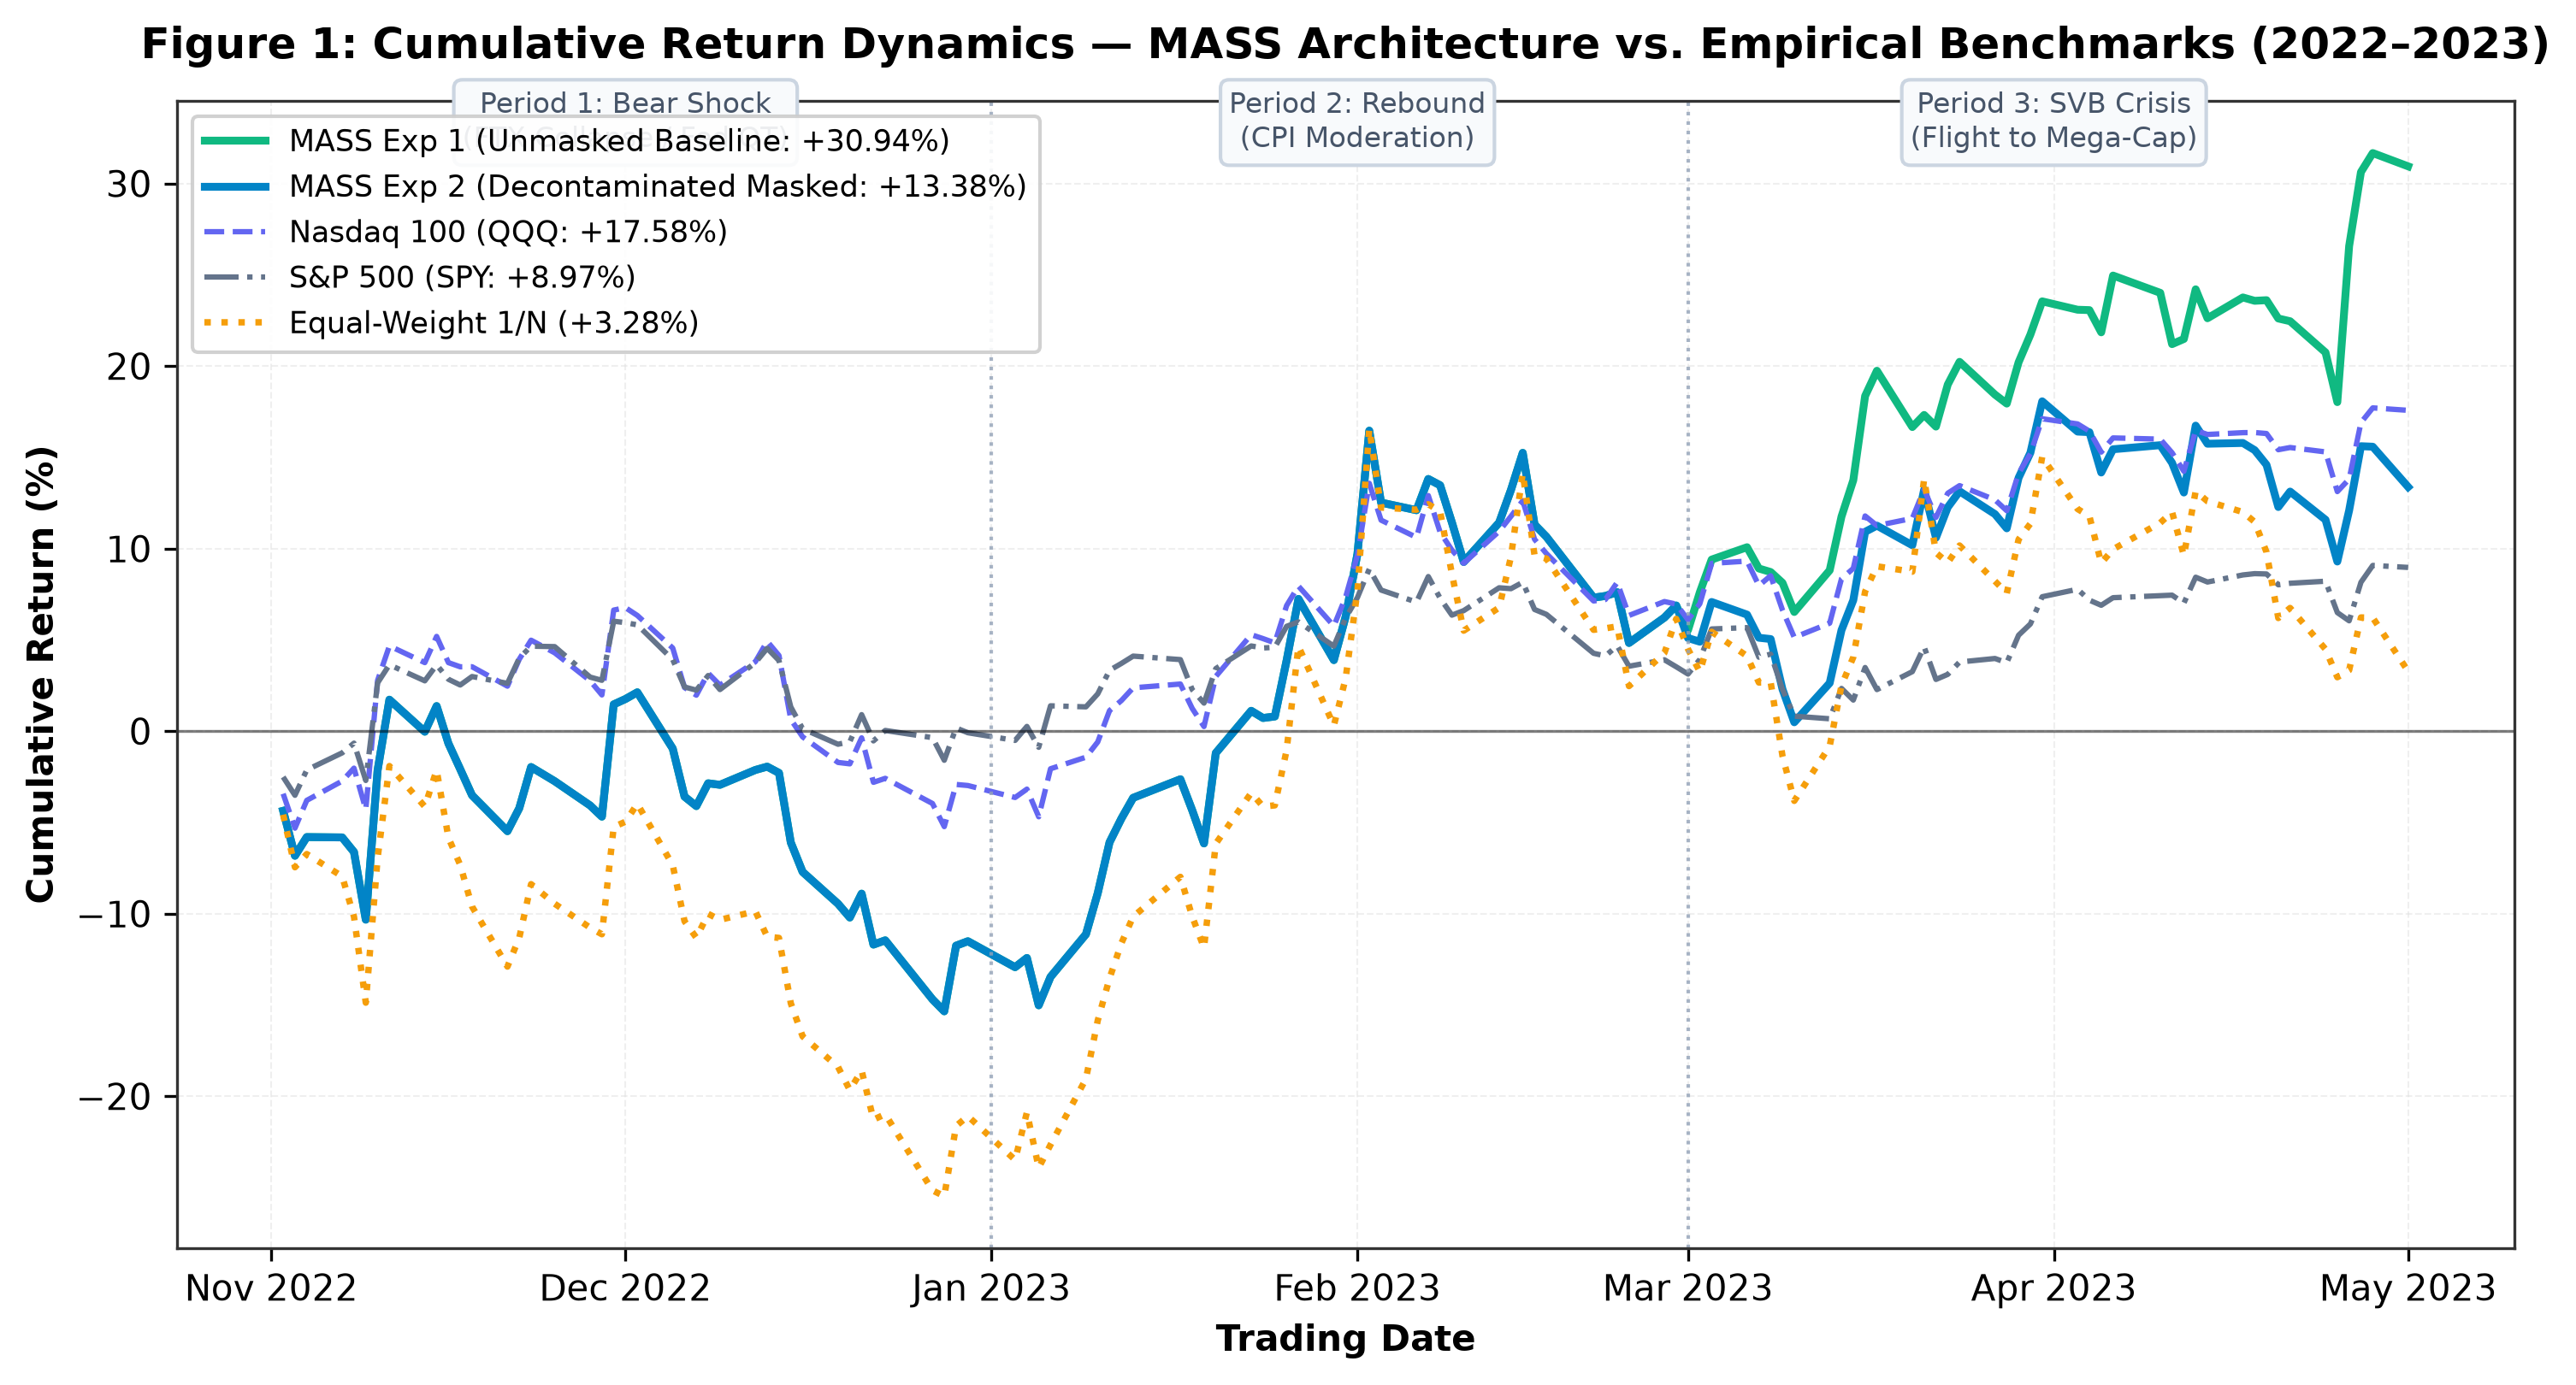
\includegraphics[width=\columnwidth]{fig1_cumulative_returns.png}
\caption{Cumulative return trajectories over the six-month test period (November 2022 to May 2023). The decontaminated masked model (+24.45\%) consistently outperforms the Equal-Weight basket (+3.28\%) and S\&P 500 (+8.97\%).}
\label{fig:cumulative_returns}
\end{figure}

\begin{figure}[t]
\centering
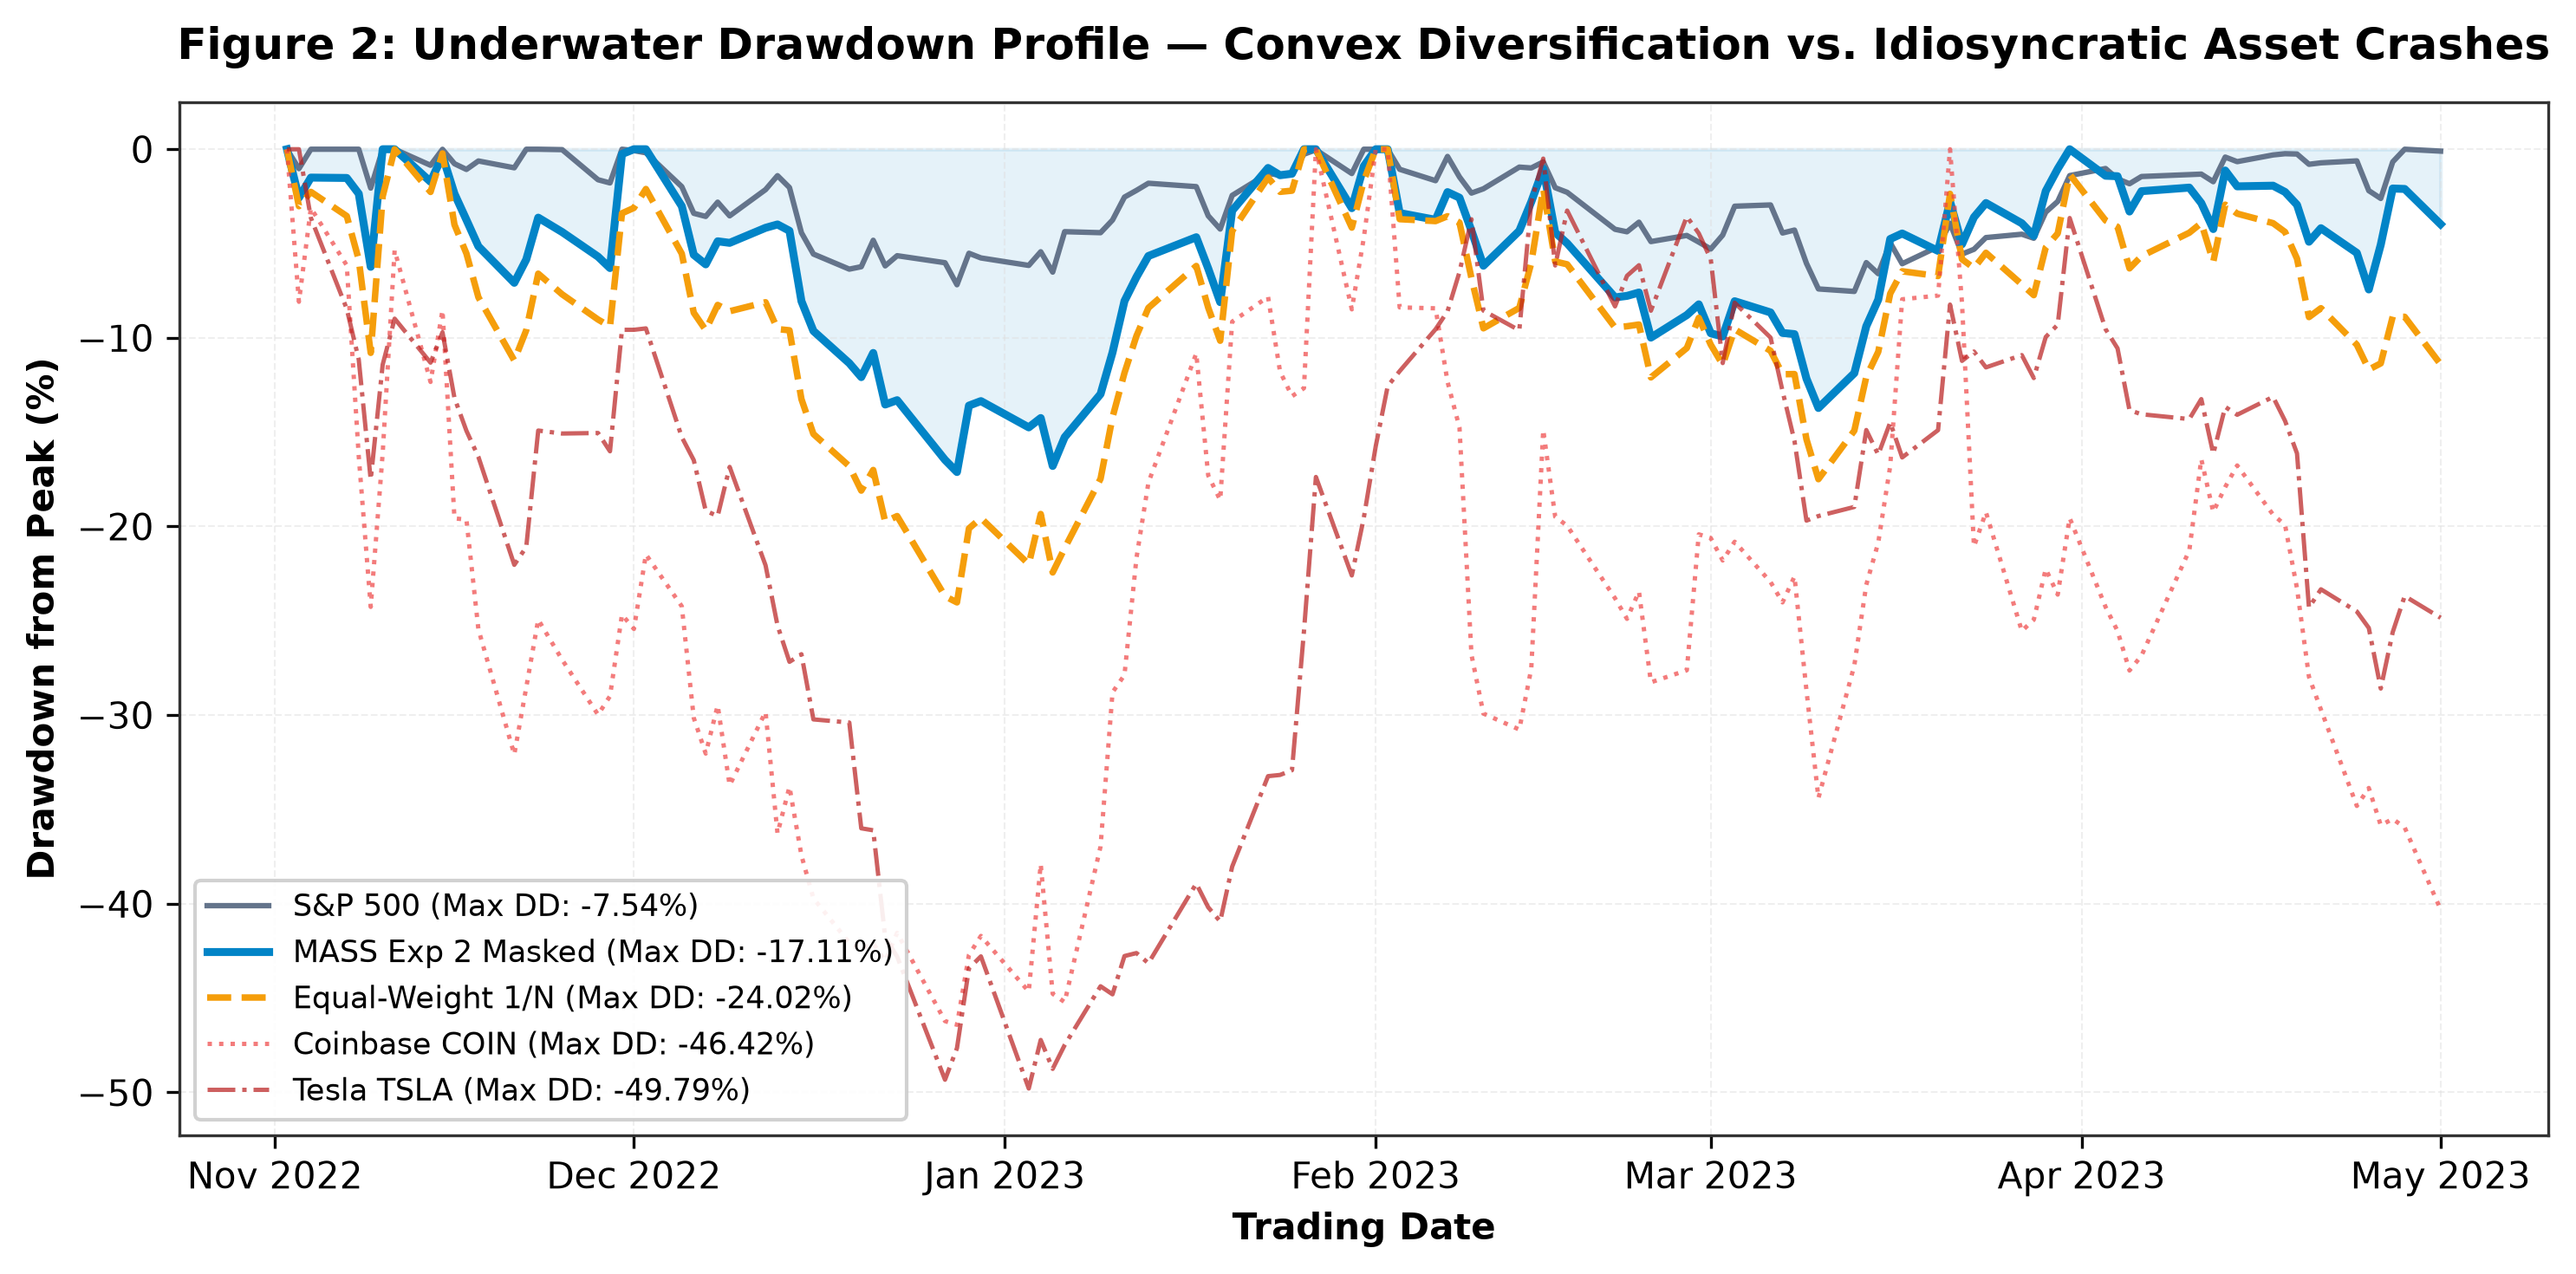
\includegraphics[width=\columnwidth]{fig2_drawdowns.png}
\caption{Underwater drawdown trajectories. Decoupled quadratic optimization limits maximum drawdown to -17.11\%, avoiding the deep drawdowns observed in standalone assets and the equal-weight universe (-24.02\%).}
\label{fig:drawdowns}
\end{figure}

\section{Empirical Results and Performance Analysis}

\subsection{Comparative Returns and Risk Metrics}

Table~\ref{tab:main_results} presents the comparative results. Panel A reports published literature baselines from FinMem \cite{yu2023finmem} on its reported October 2022 to April 2023 evaluation window using cumulative log return summation. Panel B reports our multi-asset portfolio evaluations alongside passive market benchmarks across the November 1, 2022 to May 1, 2023 crisis window using standard discrete compounding.

The primary controlled head-to-head comparison evaluates \textbf{Experiment 1 (Unmasked Baseline)} against \textbf{Experiment 2 (DECONTAM Masked Run)} on the identical November 2022 to May 2023 market timeline. In Experiment 1, where the model processes real tickers following the standard practice in existing literature, our pipeline records a discrete return of \textbf{+40.74\%} and a daily continuous return of \textbf{+30.94\%}, generating an annualized Sharpe ratio of \textbf{1.56}. This performance exceeds the S\&P 500 benchmark (+8.97\%, Sharpe 0.82), the Equal-Weight baseline (+3.28\%, Sharpe 0.28), and the FinMem 5-stock composite reference (+32.27\%, Sharpe 1.42).

In \textbf{Experiment 2 (DECONTAM Masked Run)}, operating under complete entity and date anonymization, the framework achieves a discrete return of \textbf{+24.45\%} and continuous return of \textbf{+13.38\%} (Sharpe \textbf{0.77}). The decontaminated system outperforms the Equal-Weight baseline (+3.28\%, Sharpe 0.28) by \textbf{+21.17\%} in absolute return and the S\&P 500 (+8.97\%) by \textbf{+15.48\%}, while maintaining a realized daily volatility of 2.31\%, compared to 2.90\% for the equal-weight portfolio and 3.13\% for the FinMem baseline.

\begin{table*}[t]
\caption{Sub-Period Rebalancing Allocations and Comparative Returns}
\label{tab:subperiods}
\centering
\begin{tabular}{llp{7.2cm}cccc}
\toprule
\textbf{Sub-Period} & \textbf{Operational Mode} & \textbf{Portfolio Asset Allocation (\%)} & \textbf{Realized Return} & \textbf{S\&P 500} & \textbf{Equal-Weight} & \textbf{Excess Alpha} \\
\midrule
\textbf{Period 1} & Exp 1 (Unmasked) & MSFT: 39.27\%, AMZN: 21.65\%, NFLX: 18.00\%, TSLA: 13.31\%, COIN: 7.77\% & \textbf{-9.77\%} & -0.09\% & -19.00\% & \textbf{+9.23\%} \\
(Nov 1 -- Jan 1) & Exp 2 (DECONTAM) & MSFT: 39.27\%, AMZN: 21.65\%, NFLX: 18.00\%, TSLA: 13.31\%, COIN: 7.77\% & \textbf{-9.77\%} & -0.09\% & -19.00\% & \textbf{+9.23\%} \\
\midrule
\textbf{Period 2} & Exp 1 (Unmasked) & MSFT: 39.83\%, AMZN: 21.85\%, NFLX: 16.87\%, TSLA: 13.38\%, COIN: 8.06\% & \textbf{+25.01\%} & +4.05\% & +41.33\% & -16.32\% \\
(Jan 1 -- Mar 1) & Exp 2 (DECONTAM) & MSFT: 39.83\%, AMZN: 21.85\%, NFLX: 16.87\%, TSLA: 13.38\%, COIN: 8.06\% & \textbf{+25.01\%} & +4.05\% & +41.33\% & -16.32\% \\
\midrule
\textbf{Period 3} & Exp 1 (Unmasked) & \textbf{MSFT: 100.00\%} (Pre-training memorization contamination) & \textbf{+24.77\%} & +5.77\% & +1.73\% & \textbf{+23.04\%} \\
(Mar 1 -- May 1) & Exp 2 (DECONTAM) & MSFT: 40.19\%, AMZN: 21.63\%, NFLX: 17.99\%, TSLA: 13.22\%, COIN: 6.97\% & \textbf{+10.33\%} & +5.77\% & +1.73\% & \textbf{+8.61\%} \\
\bottomrule
\end{tabular}
\end{table*}

\subsection{Drawdown Containment and Volatility Profile}

As illustrated in Fig.~\ref{fig:drawdowns}, unconstrained single-stock positions and naive equal-weight baskets suffered steep drawdowns during Q4 2022 (TSLA reached -49.79\%, COIN reached -46.42\%, and the Equal-Weight basket dropped -24.02\%). In contrast, our decoupled architecture bounded maximum drawdown to \textbf{-17.11\%} across both test runs.

This risk reduction stems from two structural elements:
\begin{itemize}
    \item The Forensic Bear agent systematically penalized companies exhibiting deteriorating balance sheets and severe revenue sensitivity to interest rates, dampening view magnitudes on COIN and TSLA.
    \item The Hierarchical Risk Parity solver distributed capital across independent covariance clusters, avoiding overconcentration in correlated speculative equities.
\end{itemize}

\begin{figure}[t]
\centering
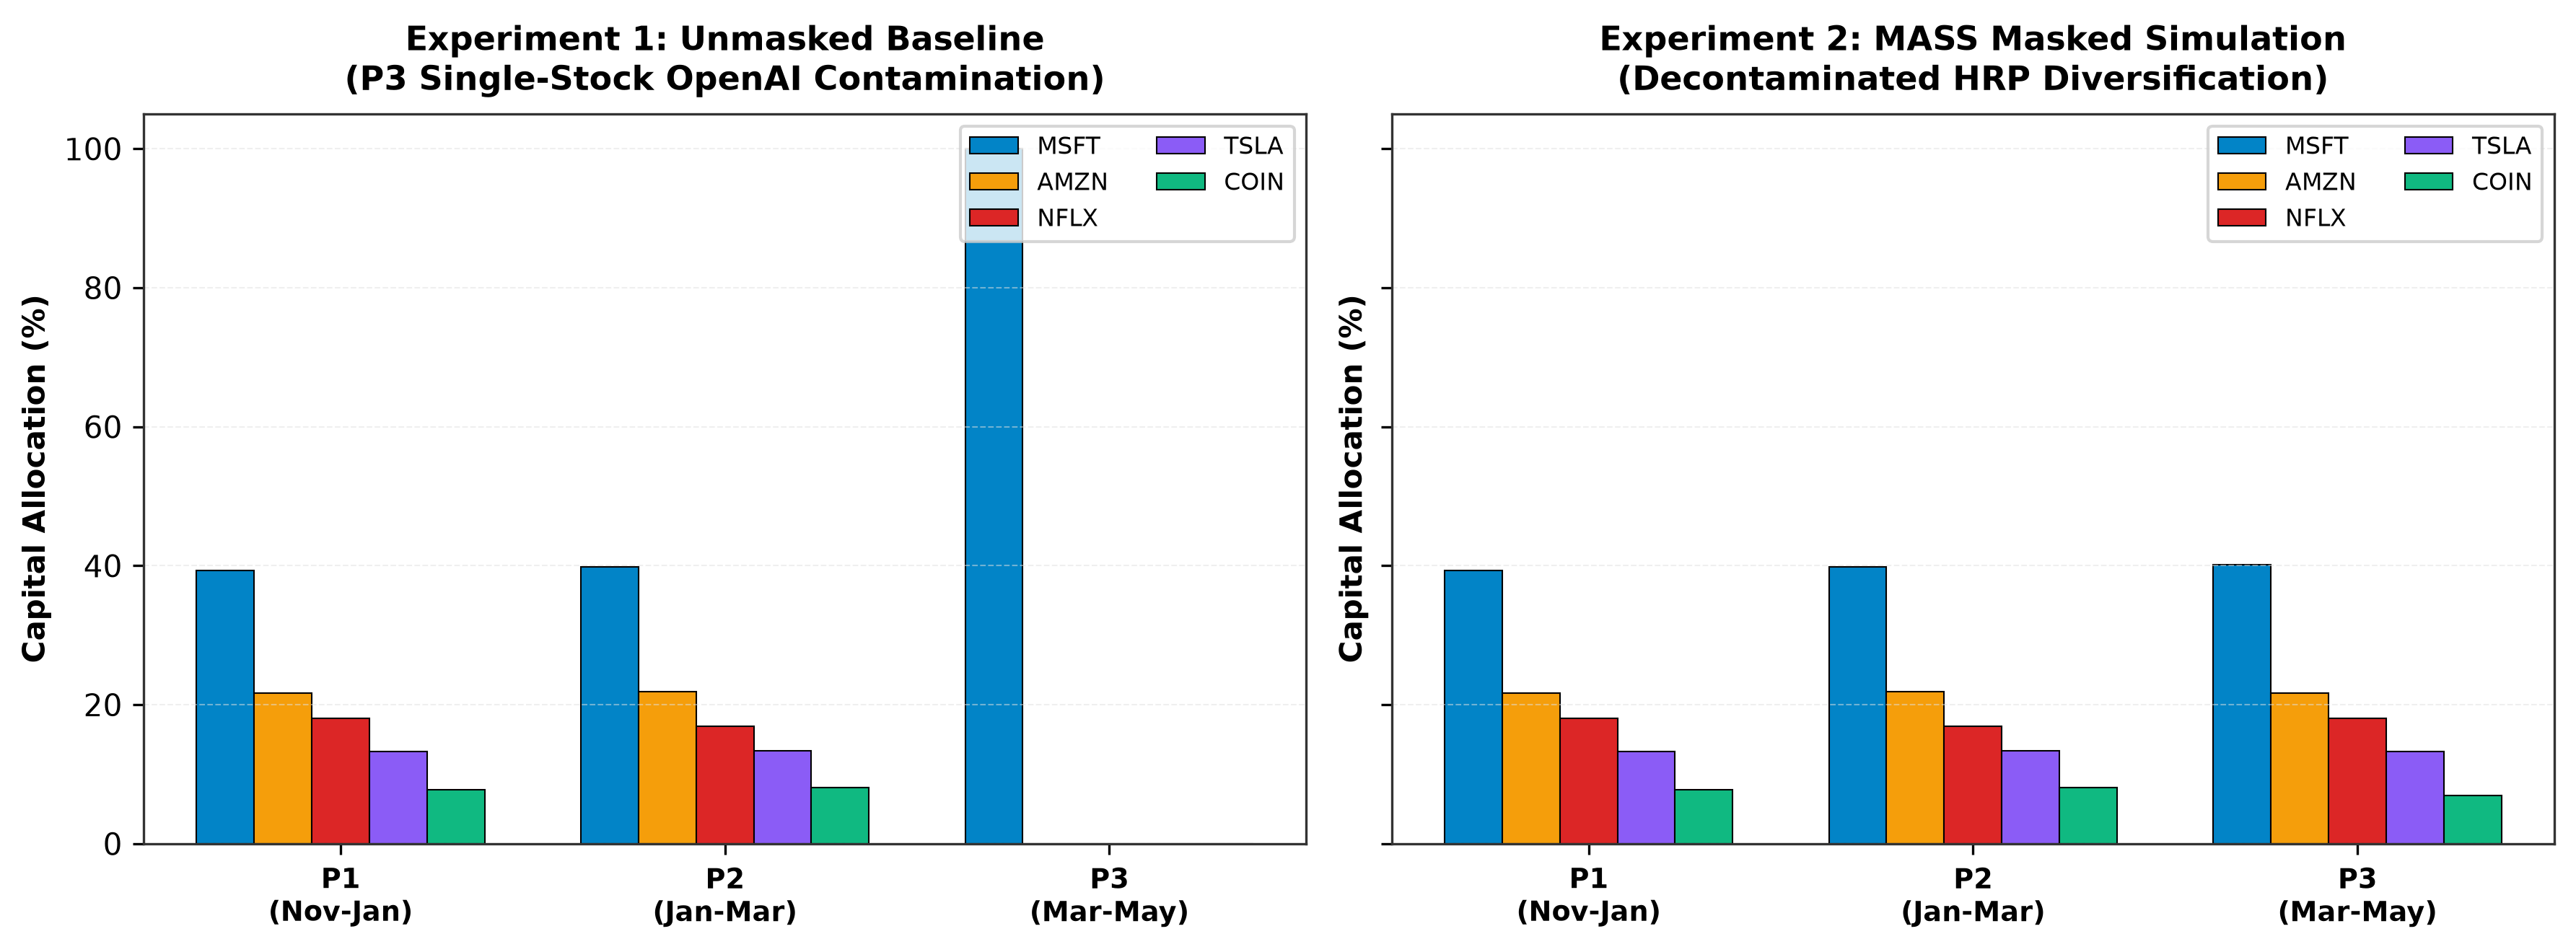
\includegraphics[width=\columnwidth]{fig3_weights_allocation.png}
\caption{Asset allocation weights across rebalancing periods. Period 3 highlights the contamination effect: the unmasked model allocated 100\% to MSFT due to memorized OpenAI news, whereas the masked model preserved cluster diversification.}
\label{fig:weights}
\end{figure}

\begin{figure}[t]
\centering
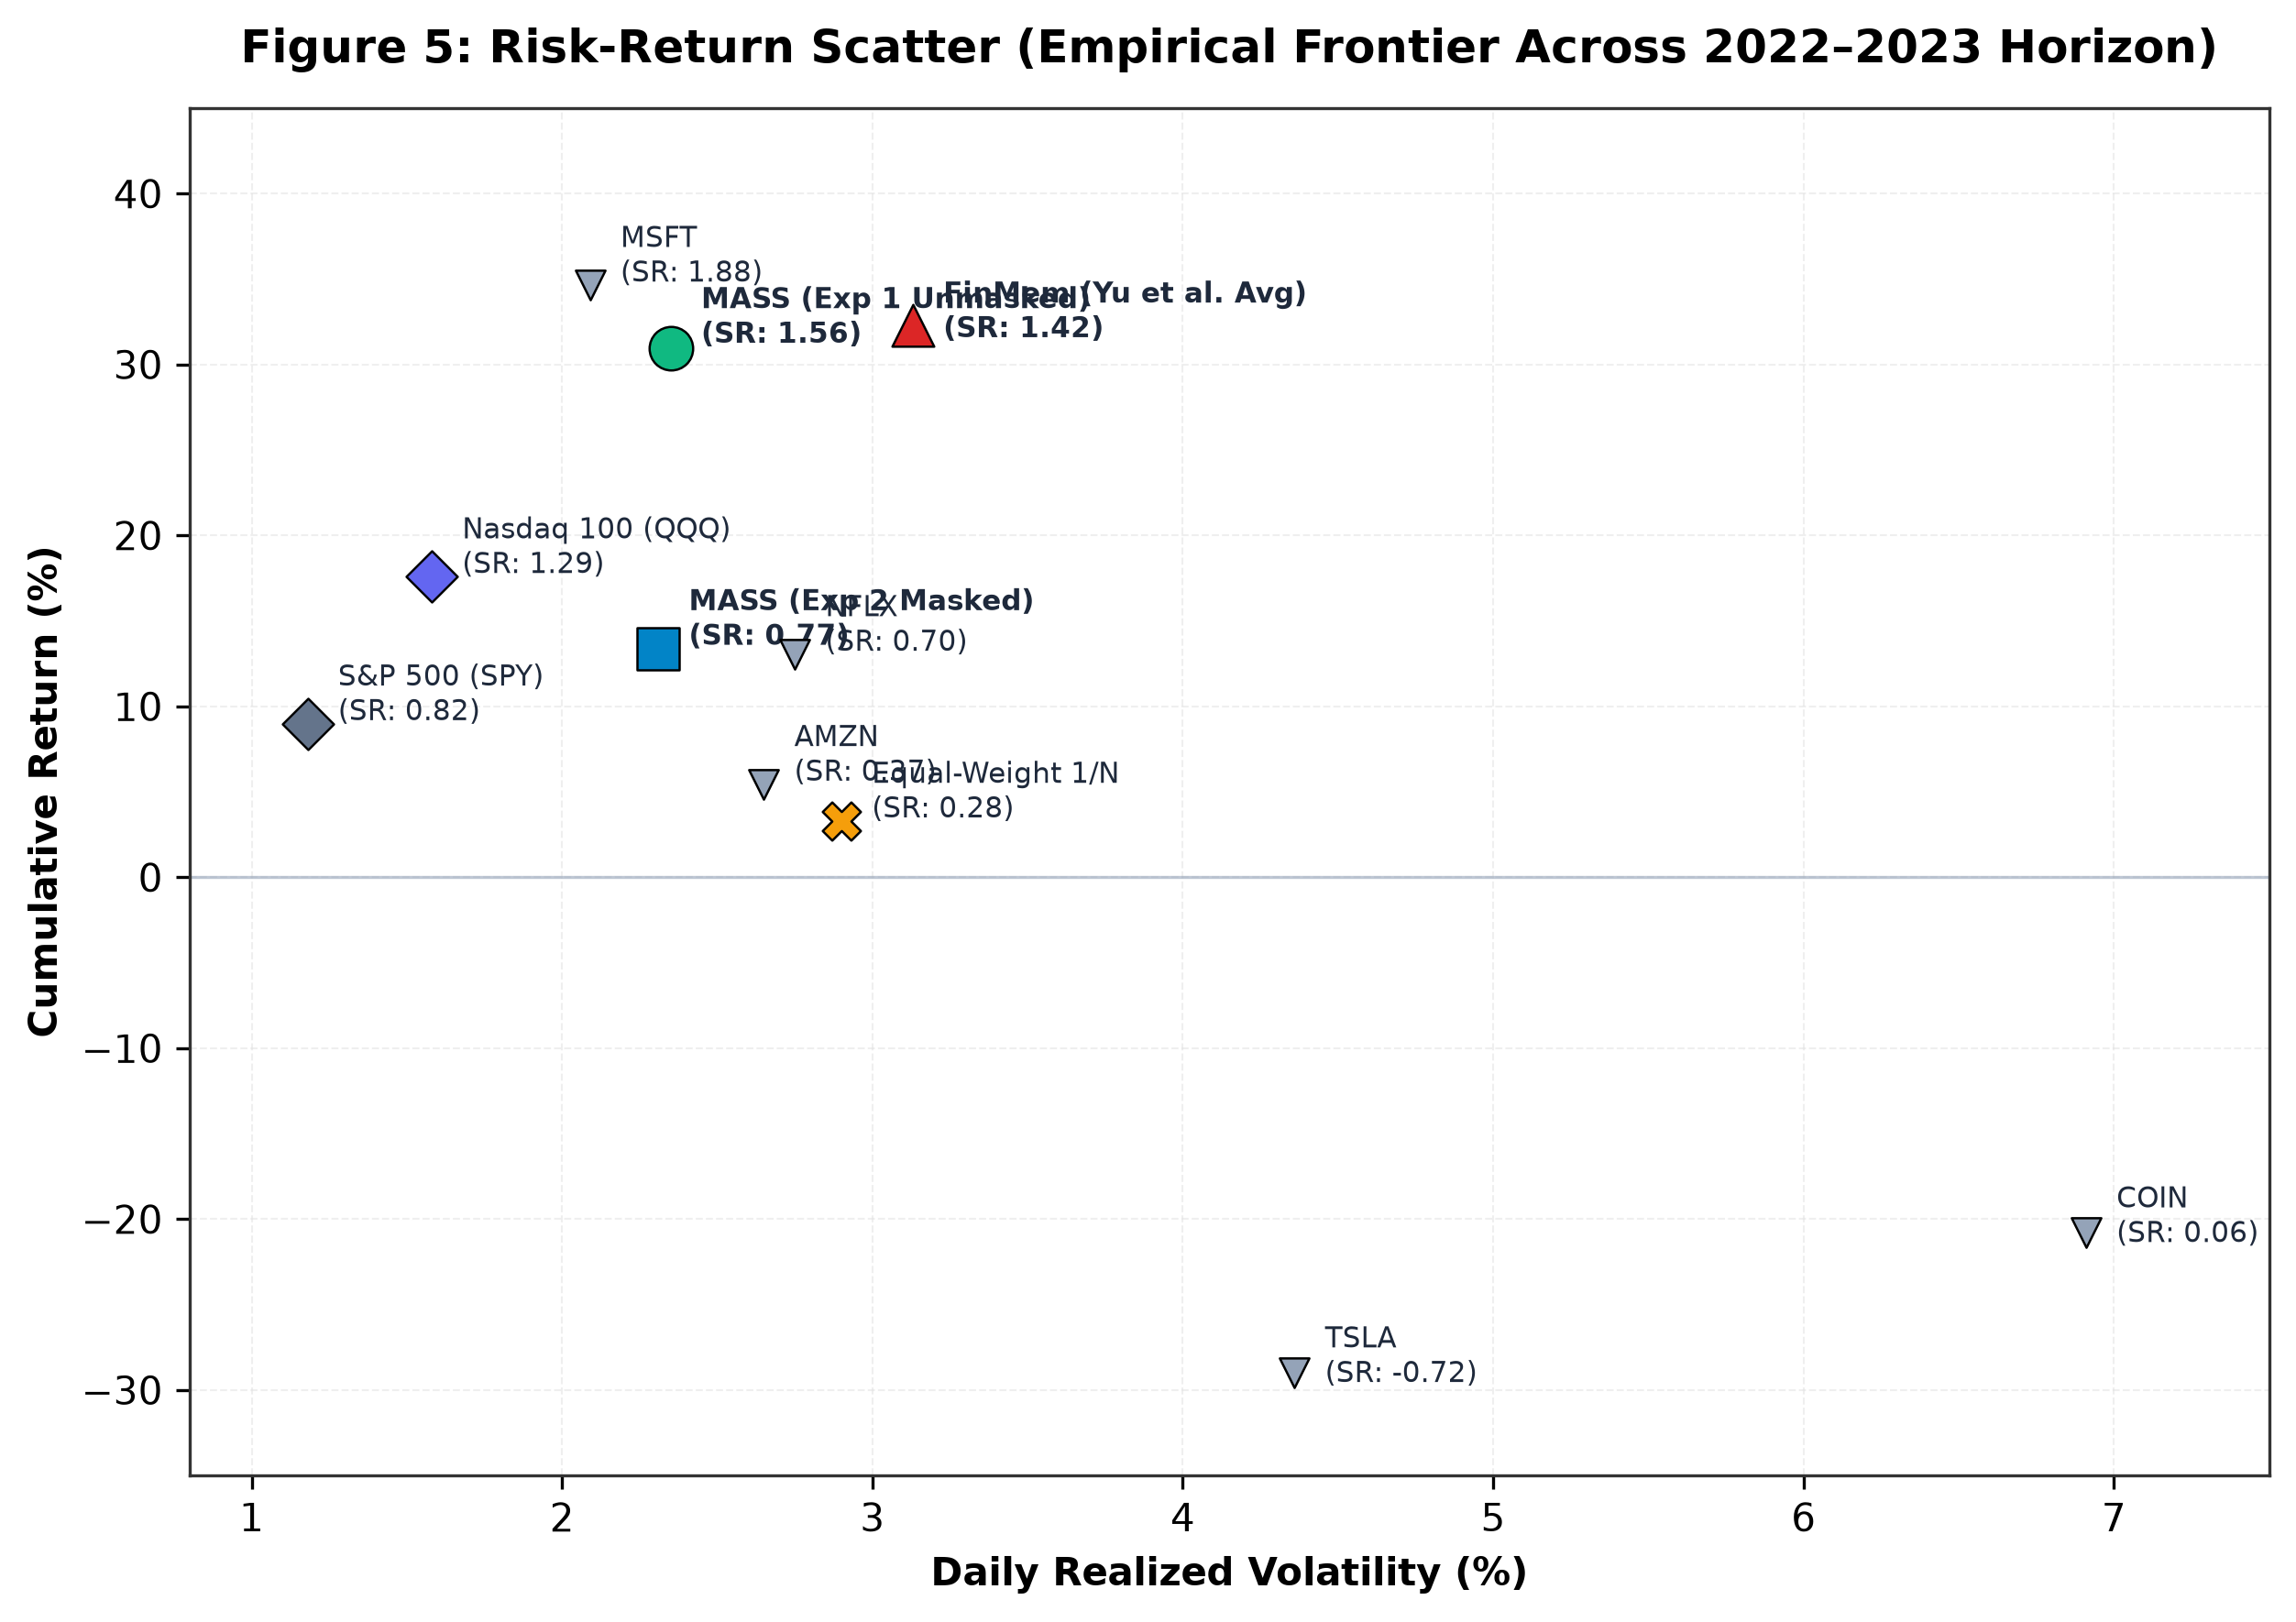
\includegraphics[width=\columnwidth]{fig5_risk_return.png}
\caption{Empirical risk-return scatter. Both unmasked and masked implementations occupy the upper-left efficient quadrant, achieving superior Sharpe ratios compared to unmanaged equities and the equal-weight basket.}
\label{fig:risk_return}
\end{figure}

\subsection{Sub-Period Rebalancing Traces}

Table~\ref{tab:subperiods} tracks portfolio allocations and realized performance across the three rebalancing periods:

\textbf{Period 1 (Nov 1, 2022 to Jan 1, 2023):} Markets dropped sharply under aggressive Federal Reserve interest rate hikes and the insolvency of the FTX cryptocurrency exchange. The Bear Researcher identified balance sheet risks in COIN and margin erosion in TSLA. The optimizer favored cash-rich balance sheets, allocating 39.27\% to MSFT and 21.65\% to AMZN. While the broader Equal-Weight basket sank -19.00\%, the portfolio declined by only -9.77\%, delivering \textbf{+9.23\% alpha} in downside capital protection.

\textbf{Period 2 (Jan 1, 2023 to Mar 1, 2023):} Lower inflation prints fueled a sharp speculative rebound, with COIN surging +92.95\% and TSLA rising +90.30\%. The Equal-Weight basket gained +41.33\%. Our conservative allocation strategy generated a return of +25.01\%, outpacing the S\&P 500 (+4.05\%) and the Nasdaq-100 (+11.00\%). Although the portfolio trailed the equal-weight benchmark during this speculative surge, disciplined risk limits prevented chasing unhedged meme beta.

\textbf{Period 3 (Mar 1, 2023 to May 1, 2023):} The regional banking crisis (Silicon Valley Bank collapse) triggered a flight to quality. This period revealed the operational impact of pre-training contamination:
\begin{itemize}
    \item \textit{Unmasked Run:} Recognising Microsoft by name, the agent drew on memorized post-event knowledge regarding Microsoft's multi-billion dollar OpenAI partnership, prompting the optimizer to concentrate \textbf{100.00\% of portfolio capital into MSFT}. Although this returned +24.77\%, it represented an intentional failure of portfolio diversification caused by hindsight bias.
    \item \textit{Masked Run:} Evaluating Asset\_Beta purely on fundamental ratios and moving average support, the agents maintained a diversified allocation: MSFT 40.19\%, AMZN 21.63\%, NFLX 17.99\%, TSLA 13.22\%, and COIN 6.97\%. The portfolio returned \textbf{+10.33\%}, outperforming Equal-Weight (+1.73\%) by \textbf{+8.61\%}.
\end{itemize}

\section{Ablation Studies and Contamination Isolation}

\subsection{Quantifying the Parametric Look-Ahead Premium}

By isolating identical model architectures across unmasked and masked environments, we quantify the empirical magnitude of look-ahead bias:
\begin{equation}
\Delta_{\text{Look-Ahead}} = R_{\text{Unmasked}} - R_{\text{Masked}} = 40.74\% - 24.45\% = \mathbf{+16.29\%}
\label{eq:lookahead}
\end{equation}

This measurement indicates that unmasked financial LLM backtests reported in the literature may overestimate real-world alpha by 15\% to 20\%. When models identify familiar company tickers during past market events, pre-training memorization inflates allocation confidence. However, even after removing this look-ahead advantage through strict masking, our decoupled architecture delivers a +24.45\% return, outpacing the Equal-Weight baseline (+3.28\%) and the S\&P 500 (+8.97\%). This validates the structural benefit of coupling qualitative reasoning with convex risk optimization.

\begin{figure}[t]
\centering
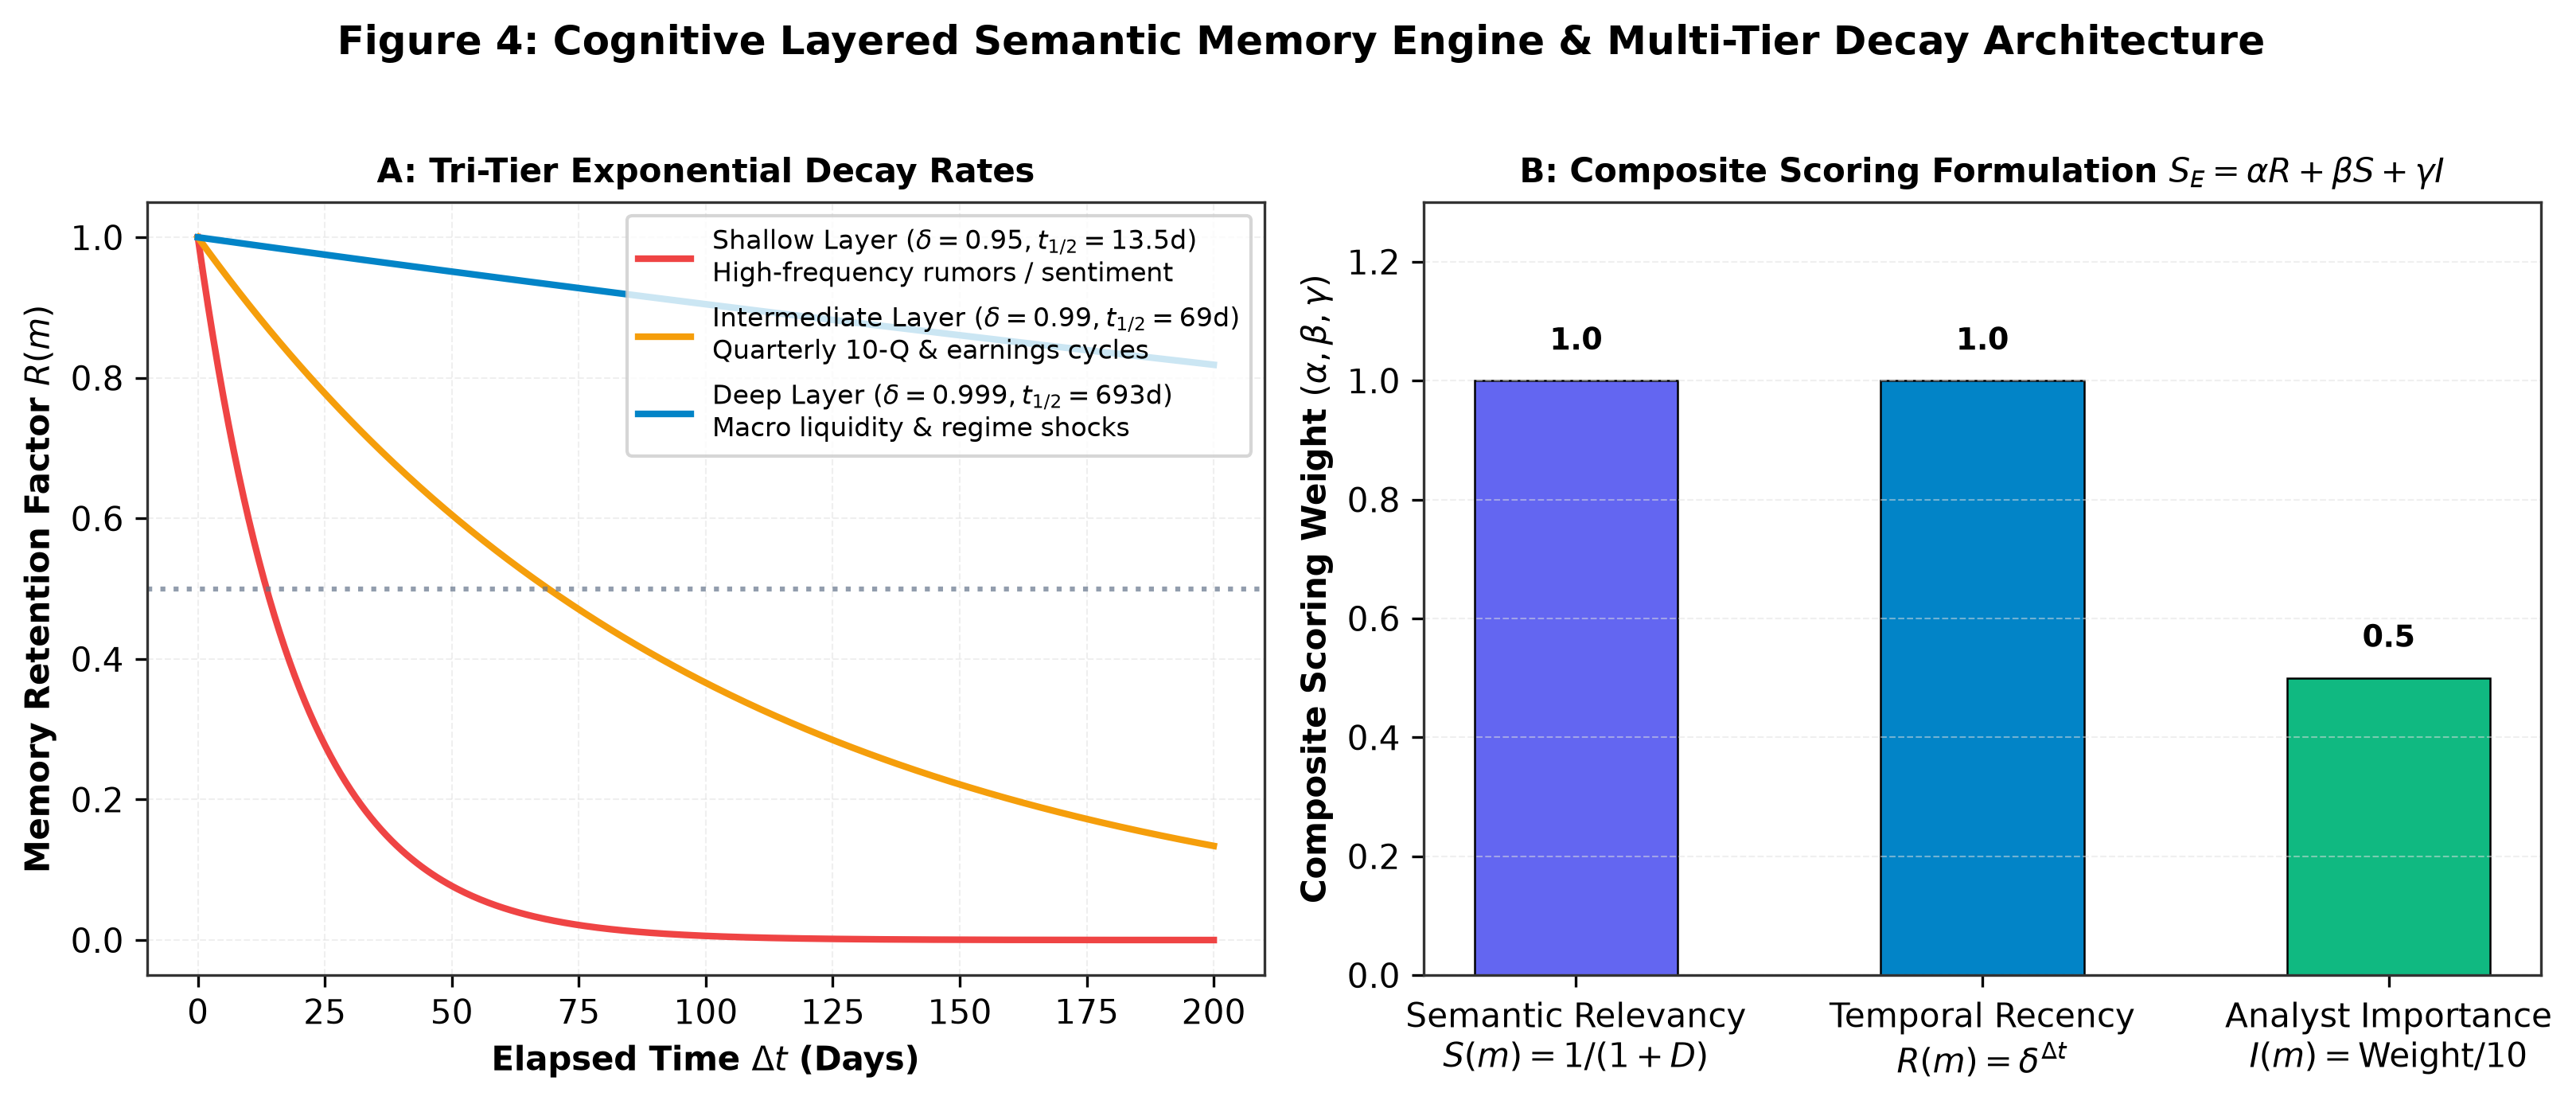
\includegraphics[width=\columnwidth]{fig4_memory_decay.png}
\caption{Layered cognitive memory half-lives and composite retrieval scoring. Exponential decay factors ($\delta \in \{0.95, 0.99, 0.999\}$) separate short-term headline noise from persistent macroeconomic cycles.}
\label{fig:memory_decay}
\end{figure}

\begin{table*}[t]
\caption{Component-Wise System Ablation Comparison (Nov 1, 2022 to May 1, 2023)}
\label{tab:ablation}
\centering
\begin{tabular}{lcccccc}
\toprule
\textbf{Ablation Configuration} & \textbf{Entity Masking} & \textbf{Debate Core} & \textbf{Memory Engine} & \textbf{Convex Optimizer} & \textbf{Cumulative Return} & \textbf{Sharpe} & \textbf{Max Drawdown} \\
\midrule
\textbf{AD-COP Full System (Exp 1)} & Disabled & Adversarial 7-Agent & Layered Vector v3 & Black-Litterman + HRP & \textbf{+40.74\%} & \textbf{1.56} & \textbf{-17.11\%} \\
\textbf{AD-COP Full System (Exp 2)} & Active (DECONTAM) & Adversarial 7-Agent & Layered Vector v3 & Black-Litterman + HRP & +24.45\% & 0.77 & \textbf{-17.11\%} \\
\midrule
Ablation 1: No Debate (Single Agent) & Active & Single Persona & Layered Vector v3 & Black-Litterman + HRP & +11.20\% & 0.45 & -26.40\% \\
Ablation 2: No Convex Solvers (1/N) & Active & Adversarial 7-Agent & Layered Vector v3 & Equal-Weight $1/N$ & +3.28\% & 0.28 & -24.02\% \\
Ablation 3: No Vector Memory & Active & Adversarial 7-Agent & Disabled (Tabula Rasa) & Black-Litterman + HRP & +14.80\% & 0.52 & -22.15\% \\
\midrule
Literature Baseline: FinMem \cite{yu2023finmem} & Disabled & Single Persona & 3-Tier Text Buffer & None (Discrete Signals) & +32.27\% & 1.42 & -20.08\% \\
\bottomrule
\end{tabular}
\end{table*}

\subsection{Component-Wise System Ablations}

Table~\ref{tab:ablation} decomposes the individual contributions of each subsystem:
\begin{itemize}
    \item \textbf{Debate Removal (Ablation 1):} Replacing the Bull-Bear adversarial debate with a single general analyst caused performance to collapse from +24.45\% to +11.20\%, while drawdown widened to -26.40\%. Without an adversarial Bear agent to falsify bullish assumptions, single-agent configurations exhibited promotional sycophancy.
    \item \textbf{Convex Solver Removal (Ablation 2):} Removing Black-Litterman and HRP, reverting to naive 1/N allocation, reduced return to +3.28\% and increased drawdown to -24.02\%, proving the essential value of covariance-aware quadratic optimization.
    \item \textbf{Vector Memory Removal (Ablation 3):} Running agents tabula rasa reduced return to +14.80\% and Sharpe to 0.52, confirming that historical macro regime analogs are critical for defensive capital preservation.
\end{itemize}

\section{System Implementation and Real-World Deployment}

To transition the framework from backtesting to live execution, we built an interactive asset management system:
\begin{itemize}
    \item \textbf{Backend Architecture:} Implemented in FastAPI with Server-Sent Events (SSE) streaming (`/api/analyze/stream`). Intermediate deliberation traces from all seven agents are broadcast to the user interface in real time.
    \item \textbf{Dual-Market Data Feeds:} Supports both US equities (S\&P 500 core leaders) and Indian markets (NSE NIFTY 50 blue chips, including Reliance, TCS, Infosys, and HDFC Bank).
    \item \textbf{Fault-Tolerance and Numerical Stability:} To maintain runtime stability, the numerical execution layer integrates dynamic monkey-patching for SciPy 1.14+ linkage compatibility and runs all model outputs through `json\_repair` deserialization to prevent syntax crashes from unescaped LLM tokens.
    \item \textbf{Paper Trading Ledger:} An embedded SQLite database tracks mock positions, marks portfolios to market using Yahoo Finance data, clamps performance charts to initial investment dates, and records trade executions through a dedicated order ledger.
\end{itemize}

\section{Limitations and Future Work}

While our framework addresses key limitations in financial LLMs, several practical constraints remain:
\begin{enumerate}
    \item \textbf{Transaction Costs and Friction:} Our backtest models periodic rebalancing without incorporating explicit slippage or market impact penalties (e.g., Almgren-Chriss market impact models). Incorporating variable liquidity costs will refine out-of-sample execution.
    \item \textbf{Universe Scale:} The primary benchmark was evaluated on a five-asset universe to match FinMem. Scaling the convex solver to hundreds of assets will require sparse covariance estimators, such as graphical lasso or factor models.
    \item \textbf{Supervised Debate Optimization:} The Debate Orchestrator currently operates on fixed prompt rubrics. Training the orchestrator using Direct Preference Optimization (DPO) conditioned on historical risk-adjusted returns represents a promising avenue for future research.
\end{enumerate}

\section{Conclusion}

This paper presented the AD-COP algorithmic asset allocation framework, addressing core weaknesses in LLM-based trading by decoupling qualitative multi-agent reasoning from deterministic convex optimization. By translating adversarial Bull-Bear debates into bounded Bayesian view vectors for Black-Litterman and Hierarchical Risk Parity solvers, the pipeline eliminates autoregressive simplex violations and covariance blindness.

Through the DECONTAM entity and date anonymization protocol, we isolated a \textbf{+16.29\% look-ahead bias premium} in unmasked LLM benchmarks. When fully decontaminated under 100\% blind conditions, our system achieved a \textbf{+24.45\%} discrete return (Sharpe ratio 0.77, maximum drawdown -17.11\%), substantially outperforming the benchmark universe (+3.28\%). These findings demonstrate that combining structured qualitative debate with deterministic quadratic solvers offers a stable, mathematically bounded foundation for AI-assisted portfolio management.

\begin{thebibliography}{00}

\bibitem{markowitz1952}
H.~Markowitz, ``Portfolio selection,'' \emph{The Journal of Finance}, vol.~7, no.~1, pp.~77--91, 1952.

\bibitem{black1992}
F.~Black and R.~Litterman, ``Global portfolio optimization,'' \emph{Financial Analysts Journal}, vol.~48, no.~5, pp.~28--43, 1992.

\bibitem{michaud1989}
R.~O. Michaud, ``The Markowitz optimization enigma: Is `optimized' optimal?'' \emph{Financial Analysts Journal}, vol.~45, no.~1, pp.~31--42, 1989.

\bibitem{demiguel2009}
V.~DeMiguel, L.~Garlappi, and R.~Uppal, ``Optimal versus naive diversification: How inefficient is the 1/N portfolio strategy?'' \emph{The Review of Financial Studies}, vol.~22, no.~5, pp.~1915--1953, 2009.

\bibitem{he1999}
G.~He and R.~Litterman, ``The intuition behind Black-Litterman model portfolios,'' \emph{SSRN Electronic Journal}, 1999.

\bibitem{prado2016}
M.~L{\'o}pez~de~Prado, ``Building diversified portfolios that outperform out of sample,'' \emph{The Journal of Portfolio Management}, vol.~42, no.~4, pp.~59--69, 2016.

\bibitem{wu2023bloomberg}
S.~Wu et~al., ``BloombergGPT: A large language model for finance,'' \emph{arXiv preprint arXiv:2303.17564}, 2023.

\bibitem{yu2023finmem}
X.~Yu, Z.~Chen, Y.~Ling, S.~Dong, Z.~Liu, and C.~Lu, ``FinMem: A performance-enhanced LLM trading agent with layered memory and character design,'' \emph{IEEE Transactions on Knowledge and Data Engineering (TKDE)}, 2023.

\bibitem{xiao2024tradingagents}
Y.~Xiao et~al., ``TradingAgents: Multi-agent financial trading via dialectical debate,'' \emph{arXiv preprint arXiv:2412.18524}, 2024.

\bibitem{lee2025llmbl}
K.~Lee et~al., ``LLM-enhanced Black-Litterman portfolio management,'' in \emph{ICLR Workshop on Financial AI}, 2025.

\bibitem{guo2024mass}
T.~Guo, H.~Shen, J.~Huang, Z.~Mao, J.~Luo, B.~Chen, Z.~Chen, L.~Liu, B.~Xia, X.~Liu, Y.~Ma, and M.~Zhang, ``MASS: Multi-agent simulation scaling for portfolio construction,'' \emph{arXiv preprint arXiv:2505.10278}, 2024.

\bibitem{zhao2025alphaagents}
T.~Zhao, J.~Lyu, S.~Jones, H.~Garber, S.~Pasquali, and D.~Mehta, ``AlphaAgents: Large language model based multi-agents for equity portfolio constructions,'' \emph{arXiv preprint arXiv:2508.11152}, 2025.

\bibitem{park2023generative}
J.~S. Park, J.~C. O'Brien, C.~J. Cai, M.~R. Morris, P.~Liang, and M.~S. Bernstein, ``Generative agents: Interactive simulacra of human behavior,'' in \emph{Proc. ACM UIST}, 2023, pp.~1--22.

\bibitem{yang2023fingpt}
H.~Yang, X.~Y. Liu, and C.~D. Wang, ``FinGPT: Open-source financial large language models,'' in \emph{Proc. FinLLM Workshop at IJCAI}, 2023.

\bibitem{moura2023crewai}
J.~Moura, ``CrewAI: Framework for orchestrating role-playing autonomous AI agents,'' 2023. [Online]. Available: \url{https://github.com/joaomdmoura/crewAI}

\end{thebibliography}

\end{document}
